\documentclass[12pt,a4paper]{article}

% \usepackage[utf8]{inputenc}
% \DeclareUnicodeCharacter{1D12A}{\doublesharp}
% \DeclareUnicodeCharacter{2693}{\anchor}
% \usepackage{dingbat}
% \DeclareRobustCommand\dash\unskip\nobreak\thinspace{\textemdash\allowbreak\thinspace\ignorespaces}
\usepackage[top=1in, bottom=1in, left=1in, right=1in, headheight=15pt]{geometry}
%\usepackage{fullpage}

\usepackage{tabularx}
\usepackage{multirow}
\usepackage{makecell}
\usepackage{fancyhdr}\pagestyle{fancy}\rhead{Stephanie Wang}\lhead{SIAM Travel Award Application Statement}

\usepackage{amsmath,amssymb,amsthm,amsfonts,microtype,stmaryrd,mathtools}
	%{wasysym,yhmath}

\usepackage[usenames,dvipsnames]{xcolor}
\newcommand{\blue}[1]{\textcolor{blue}{#1}}
\newcommand{\red}[1]{\textcolor{red}{#1}}
\newcommand{\gray}[1]{\textcolor{gray}{#1}}
\newcommand{\fgreen}[1]{\textcolor{ForestGreen}{#1}}

\usepackage{mdframed}
	%\newtheorem{mdexample}{Example}
	\definecolor{warmgreen}{rgb}{0.8,0.9,0.85}
	% --Example:
	% \begin{center}
	% \begin{minipage}{0.7\textwidth}
	% \begin{mdframed}[backgroundcolor=warmgreen, 
	% skipabove=4pt,skipbelow=4pt,hidealllines=true, 
	% topline=false,leftline=false,middlelinewidth=10pt, 
	% roundcorner=10pt] 
	%%%% --CONTENTS-- %%%%
	% \end{mdframed}\end{minipage}\end{center}	

\usepackage{graphicx} \graphicspath{{}}
	% --Example:
	% \includegraphics[scale=0.5]{picture name}
%\usepackage{caption} %%% --some awful package to make caption...

\usepackage[unicode]{hyperref}\hypersetup{linktocpage,colorlinks}\hypersetup{citecolor=black,filecolor=black,linkcolor=black,urlcolor=blue,breaklinks=true}

%%% --Text Fonts
%\usepackage{times} %%% --Times New Roman for LaTeX
%\usepackage{fontspec}\setmainfont{Times New Roman} %%% --Times New Roman; XeLaTeX only

%%% --Math Fonts
\renewcommand{\v}[1]{\ifmmode\mathbf{#1}\fi}
\renewcommand{\b}[1]{\ifmmode\boldsymbol{#1}\fi}
%\renewcommand{\mbf}[1]{\mathbf{#1}} %%% --vector
%\newcommand{\ca}[1]{\mathcal{#1}} %%% --"bigO"
%\newcommand{\bb}[1]{\mathbb{#1}} %%% --"Natural, Real numbers"
%\newcommand{\rom}[1]{\romannumeral{#1}} %%% --Roman numbers

%%% --Quick Arrows
\newcommand{\ra}[1]{\ifnum #1=1\rightarrow\fi\ifnum #1=2\Rightarrow\fi\ifnum #1=3\Rrightarrow\fi\ifnum #1=4\rightrightarrows\fi\ifnum #1=5\rightleftarrows\fi\ifnum #1=6\mapsto\fi\ifnum #1=7\iffalse\fi\fi\ifnum #1=8\twoheadrightarrow\fi\ifnum #1=9\rightharpoonup\fi\ifnum #1=0\rightharpoondown\fi}

%\newcommand{\la}[1]{\ifnum #1=1\leftarrow\fi\ifnum #1=2\Leftarrow\fi\ifnum #1=3\Lleftarrow\fi\ifnum #1=4\leftleftarrows\fi\ifnum #1=5\rightleftarrows\fi\ifnum #1=6\mapsfrom\ifnum #1=7\iffalse\fi\fi\ifnum #1=8\twoheadleftarrow\fi\ifnum #1=9\leftharpoonup\fi\ifnum #1=0\leftharpoondown\fi}

%\newcommand{\ua}[1]{\ifnum #1=1\uparrow\fi\ifnum #1=2\Uparrow\fi}
%\newcommand{\da}[1]{\ifnum #1=1\downarrow\fi\ifnum #1=2\Downarrow\fi}

%%% --Special Editor Config
\renewcommand{\ni}{\noindent}
\newcommand{\onum}[1]{\raisebox{.5pt}{\textcircled{\raisebox{-1pt} {#1}}}}

\newcommand{\claim}[1]{\underline{``{#1}":}}

\renewcommand{\l}{\left}\renewcommand{\r}{\right}\newcommand{\m}{\middle}

\newcommand{\casebrak}[4]{\left \{ \begin{array}{ll} {#1},&{#2}\\{#3},&{#4} \end{array} \right.}
%\newcommand{\ttm}[4]{\l[\begin{array}{cc}{#1}&{#2}\\{#3}&{#4}\end{array}\r]} %two-by-two-matrix
%\newcommand{\tv}[2]{\l[\begin{array}{c}{#1}\\{#2}\end{array}\r]}

\def\dps{\displaystyle}

\let\italiccorrection=\/
\def\/{\ifmmode\expandafter\frac\else\italiccorrection\fi}


%%% --General Math Symbols
\def\bc{\because}
\def\tf{\therefore}

%%% --Frequently used OPERATORS shorthand
\newcommand{\INT}[2]{\int_{#1}^{#2}}
\newcommand{\Int}[1]{\int_{#1}}
% \newcommand{\UPINT}{\bar\int}
% \newcommand{\UPINTRd}{\overline{\int_{\bb R ^d}}}
\newcommand{\SUM}[2]{\sum\limits_{#1}^{#2}}
\newcommand{\PROD}[2]{\prod\limits_{#1}^{#2}}
\newcommand{\CUP}[2]{\bigcup\limits_{#1}^{#2}}
\newcommand{\CAP}[2]{\bigcap\limits_{#1}^{#2}}
% \newcommand{\SUP}[1]{\sup\limits_{#1}}
% \newcommand{\INF}[1]{\inf\limits_{#1}}
\newcommand{\pd}[2]{\frac{\partial{#1}}{\partial{#2}}}
\def\tr{\text{tr}}

\renewcommand{\o}{\circ}
\newcommand{\x}{\times}
\newcommand{\ox}{\otimes}

\newcommand\ie{{\it i.e. }}
\newcommand\wrt{{w.r.t. }}
\newcommand\dom{\mathbf{dom\:}}

%%% --Frequently used VARIABLES shorthand
\newcommand{\R}{\ifmmode\mathbb R\fi}
\newcommand{\N}{\ifmmode\mathbb N\fi}
\newcommand{\T}{\ifmmode\mathbb T\fi}
\renewcommand{\O}{\mathcal{O}}
\newcommand{\w}{\wedge}
\newcommand{\ome}{\omega}
\newcommand{\lam}{\lambda}
\newcommand{\im}{\mbox{im}}

\newcommand{\B}{\mathcal B}

%============================
% Conjugate, Double bracket
%============================

\makeatletter
\DeclareFontFamily{OMX}{MnSymbolE}{}
\DeclareSymbolFont{MnLargeSymbols}{OMX}{MnSymbolE}{m}{n}
\SetSymbolFont{MnLargeSymbols}{bold}{OMX}{MnSymbolE}{b}{n}
\DeclareFontShape{OMX}{MnSymbolE}{m}{n}{
    <-6>  MnSymbolE5
   <6-7>  MnSymbolE6
   <7-8>  MnSymbolE7
   <8-9>  MnSymbolE8
   <9-10> MnSymbolE9
  <10-12> MnSymbolE10
  <12->   MnSymbolE12
}{}
\DeclareFontShape{OMX}{MnSymbolE}{b}{n}{
    <-6>  MnSymbolE-Bold5
   <6-7>  MnSymbolE-Bold6
   <7-8>  MnSymbolE-Bold7
   <8-9>  MnSymbolE-Bold8
   <9-10> MnSymbolE-Bold9
  <10-12> MnSymbolE-Bold10
  <12->   MnSymbolE-Bold12
}{}
\let\llangle\@undefined
\let\rrangle\@undefined
\DeclareMathDelimiter{\llangle}{\mathopen}%
                     {MnLargeSymbols}{'164}{MnLargeSymbols}{'164}
\DeclareMathDelimiter{\rrangle}{\mathclose}%
                     {MnLargeSymbols}{'171}{MnLargeSymbols}{'171}
\makeatother

\title{SIAM Travel Award Application Statement}
\author{Stephanie Wang}
\date{\today}

% The following lines include both bibentry and hyperref packages while resolving the clash
% See https://tex.stackexchange.com/questions/65348/clash-between-bibentry-and-hyperref-with-bibstyle-elsart-harv
\usepackage{bibentry} % using BibTeX for publication list
\makeatletter\let\saved@bibitem\@bibitem\makeatother

\begin{document}
I am hereby applying for SIAM Travel Award to fund my travel to Tokyo in August of 2023 to present my paper \href{https://dl.acm.org/doi/10.1145/3450626.3459781}{Computing minimal surfaces with differential forms} at the 10th International Congress on Industrial and Applied Mathematics.  
My talk will be a part of the ``Computational methods for interfaces in physics and mechanics'' (numbered 00690) minisymposium, organized by \href{http://www.cmap.polytechnique.fr/~antonin/}{Prof. Antonin Chambolle} and \href{https://ms.mcmaster.ca/~bourdinb/}{Prof. Blaise Bourdin}.  
In the aforementioned paper, my co-author and I explored a new numerical representation of geometries called \emph{current}, which originated from the study of geometric measure theory (GMT).  
Existing geometry representations either explicitly store positions of the vertices and a combinatorial structure of the connectivity, or implicitly encode the geometries as the level set of a function, lacking the capacity to represent geometries with nonempty boundaries.  
Our GMT-based representation simultaneously provides the capacity of representing geometries with boundaries as well as the convenience of continuous and differentiable changes in topology.  
We demonstrate in our paper how this new geometry representation turns the nonconvex Plateau problem into a textbook convex problem-- a convex, norm-like functional to minimize, along with a linear constraint.  
Our computational method utilizes the recent development of Alternating Direction Method of Multipliers (ADMM) and Fast Fourier Transform (FFT), making the minimization process both fast and robust.  
In addition, I will also cover an extended work in my talk, \href{https://openaccess.thecvf.com/content/CVPR2022/papers/Palmer_DeepCurrents_Learning_Implicit_Representations_of_Shapes_With_Boundaries_CVPR_2022_paper.pdf}{DeepCurrents: Learning Implicit Representations of Shapes with Boundaries}, where my co-authors and I used Fourier features together with deep neural network to discretize currents to achieve infinite resolution as well as a data-driven auto-encoder of surfaces with boundaries. 

The GMT-based geometry representation has a lot of potential for future computational methods, for its flexibility with topology changes, differentiability, and an easy linear operator to compute the boundaries.  
I am hoping to exchange ideas with other mathematicians working in computational methods in physics as well as mechanics.  
Attached below are rendered images of our computational results of Plateau problems. 
I appreciate SIAM's consideration of my application, and I look forward to hearing from the award committee. 
\begin{figure*}[h]
  \centering
    \includegraphics[width=0.4\linewidth]{Borromean_DGD_calendar_powerplant_blue.png}
    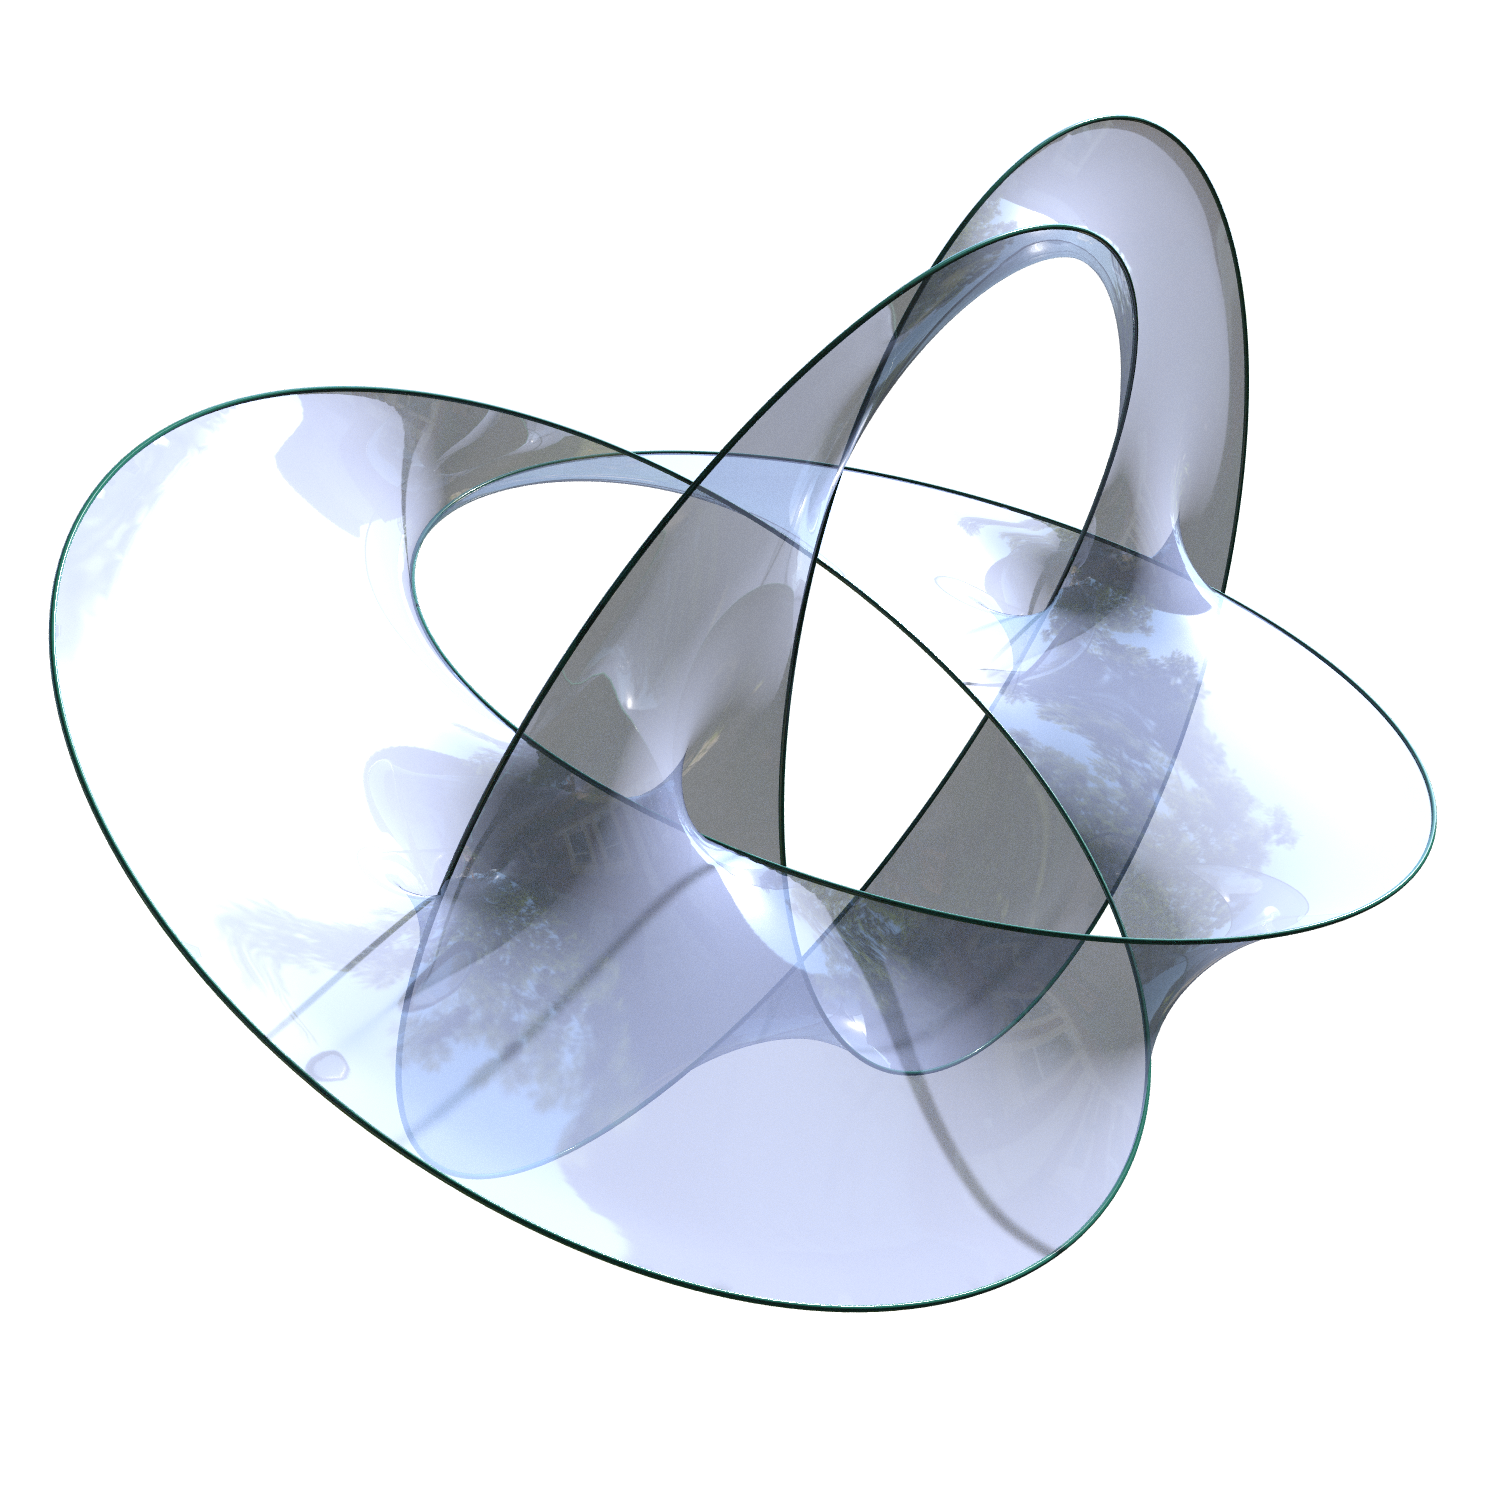
\includegraphics[width=0.4\linewidth]{DGD_calendar_collage_rings_surface.png}
    \caption{
      Predicting the topology of the solution to Plateau problem has always been a difficult problem. Our computational method can handle arbitrary boundary curves and always find the global minimizer for Plateau problem. Left: minimal surface with boundary prescribed as the Borromean rings (prescribed in squared shapes). Right: minimal surface with boundary prescribed as five arbitrarily positioned circles. 
    }
  \end{figure*}

\end{document}
